
% Arquivo de origem: cap_funcao/cap_funcao.tex
% Arquivo de destino: cap_funcao/figs/tikz/figura_cap_funcao_1.tex
% Processamento: 07/15/22 - 14:24:29
\documentclass[crop,tikz,convert=pdf2svg]{standalone}
\usetikzlibrary{fit,shapes.geometric,arrows} 
\begin{document}
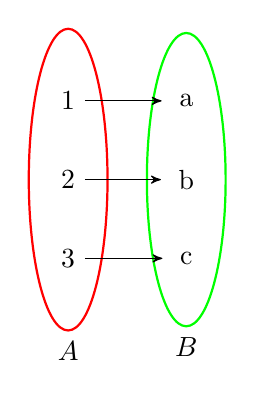
\begin{tikzpicture}[scale=0.50]
 \node (1) at (0,0) {1};%\filldraw(1.east) circle (1pt)
 \node (2) [below of=1] {2};%\filldraw(2.east) circle (1pt)
 \node (3) [below of=2] {3};%\filldraw(3.east) circle (1pt)
 \node[fit=(1) (2) (3),ellipse,draw=red,minimum width=1cm,thick,label=below:\(A\)]{};

 \node (a) at (3,0) {a};%\filldraw($b_1$.west) circle (1pt)
 \node (b) [below of=a] {b};%\filldraw($b_2$.west) circle (1pt)
 \node (c) [below of=b] {c};%\filldraw($b_3$.west) circle (1pt)
 \node[fit=(a) (b) (c),ellipse,draw=green,minimum width=1cm,thick,label=below:\(B\)]{};

 \draw[->, shorten >=.1cm, >=stealth'] (1.east) to (a.west);
 \draw[->, shorten >=.1cm, >=stealth'] (2.east) to (b.west);
 \draw[->, shorten >=.1cm, >=stealth'] (3.east) to (c.west);
\end{tikzpicture}
\end{document}
